% Supplementary Materials for the Applied Sciences submission.
\documentclass[applsci,supfile,submit,pdftex,moreauthors]{Definitions/mdpi}

\usepackage{graphicx}
\usepackage{etoolbox}
\usepackage{amsfonts}
\usepackage{booktabs}
\usepackage{multirow}
\usepackage{array}
\usepackage{tabularx}
\usepackage{listings}
\usepackage{tikz}
\usepackage{pgfplots}
\usepackage{xspace}
\usepackage{placeins}
\usepackage{xr}

\externaldocument[M-]{main}
\usetikzlibrary{arrows.meta,backgrounds,calc,fit,matrix,positioning,shapes.geometric}
\pgfplotsset{compat=1.18}
\definecolor{prblue}{HTML}{2F6B9A}
\definecolor{prteal}{HTML}{2A9D8F}
\definecolor{prgold}{HTML}{E9A23B}
\definecolor{prred}{HTML}{C9574D}
\definecolor{prpurple}{HTML}{7768AE}
\definecolor{prgray}{HTML}{5D6670}
\definecolor{prlightblue}{HTML}{EAF2F8}
\definecolor{prlightteal}{HTML}{E8F5F2}
\definecolor{prlightgold}{HTML}{FCF3E4}
\definecolor{prlightred}{HTML}{F9ECEA}
\newcolumntype{Y}{>{\raggedright\arraybackslash}X}
\newcommand{\model}{\textsc{ProcRosetta}\xspace}
\newcommand{\best}[1]{\textbf{#1}}
\renewcommand{\thefigure}{S\arabic{figure}}
\renewcommand{\thetable}{S\arabic{table}}
\setlength{\headheight}{20pt}

\firstpage{1}
\pubvolume{16}
\issuenum{1}
\articlenumber{0}
\pubyear{2026}
\doinum{}
\Title{ProcRosetta: Behavior-Supervised Alignment and Retrieval of Heterogeneous Process Mining Artifacts}
\Author{Alessandro Berti $^{1,*}$ and Wil M. P. van der Aalst $^{1,2}$}
\AuthorNames{Alessandro Berti and Wil M. P. van der Aalst}
\address{$^{1}$ Process and Data Science Group, RWTH Aachen University, Aachen, Germany; $^{2}$ Celonis, Munich, Germany}
\corres{Correspondence: a.berti@pads.rwth-aachen.de}

\begin{document}

\section{Generator schematics}\label{app:generator-schematics}

Figure~\ref{fig:tree-sampler} separates recursive topology construction from acceptance of the folded decoder target. Figure~\ref{fig:row-expansion} then shows how one accepted family becomes four rows without crossing a split boundary.

\begin{figure}[H]
\centering
\resizebox{0.94\textwidth}{!}{%
\begin{tikzpicture}[
 flowbox/.style={draw=prgray!70,rounded corners=2pt,align=center,minimum height=10mm,text width=27mm,inner sep=3pt},
 flowdecision/.style={diamond,draw=prgray!70,aspect=2.0,align=center,text width=17mm,inner sep=1pt},
 flowarrow/.style={-{Stealth[length=1.7mm]},semithick,draw=prblue}
]
\node[flowbox,fill=prlightgold] (root) at (0,0) {plan root operator};
\node[flowbox,fill=prlightteal] (topology) at (3.6,0) {sample unlabeled topology};
\node[flowdecision,fill=prlightgold] (capacity) at (7.0,0) {activity capacity?};
\node[flowbox,fill=prlightblue] (labels) at (10.2,0) {assign activities after topology};
\node[flowbox,fill=prlightblue] (fold) at (13.8,0) {canonicalize, fold, and measure};
\node[flowdecision,fill=prlightgold] (profile) at (17.2,0) {ordinary profile met?};
\node[flowbox,fill=prlightteal] (accept) at (20.4,0) {accept decoder target};
\node[flowbox,fill=prlightred] (retry) at (13.8,-2.3) {reject candidate};
\node[flowbox,fill=prlightred] (error) at (18.8,-2.3) {attempt budget exhausted: error};
\draw[flowarrow] (root)--(topology);
\draw[flowarrow] (topology)--(capacity);
\draw[flowarrow] (capacity)--node[above,font=\scriptsize]{yes}(labels);
\draw[flowarrow] (labels)--(fold);
\draw[flowarrow] (fold)--(profile);
\draw[flowarrow] (profile)--node[above,font=\scriptsize]{yes}(accept);
\draw[flowarrow] (capacity.south) |- node[pos=0.25,left,font=\scriptsize]{no} (retry.west);
\draw[flowarrow] (profile.south) |- node[pos=0.25,right,font=\scriptsize]{no} (retry.east);
\draw[flowarrow] (retry)--(error);
\draw[flowarrow] (retry.south) to[out=-90,in=-90,looseness=1.4]
  node[below,font=\scriptsize]{attempt remains} (topology.south);
\end{tikzpicture}%
}
\caption{Topology-first sampling for ordinary families. Activity requirements are checked without padding, and acceptance is based on the folded target seen by the decoder.}
\label{fig:tree-sampler}
\end{figure}

\begin{figure}[H]
\centering
\resizebox{0.94\textwidth}{!}{%
\begin{tikzpicture}[
 familybox/.style={draw=prgray!70,rounded corners=2pt,fill=prlightgold,align=center,minimum height=18mm,text width=32mm},
 viewbox/.style={draw=prgray!70,rounded corners=2pt,fill=prlightblue,align=center,minimum height=11mm,text width=25mm},
 mapbox/.style={draw=prgray!70,rounded corners=2pt,fill=prlightteal,align=center,minimum height=11mm,text width=29mm},
 rowbox/.style={draw=prgray!70,rounded corners=2pt,fill=white,align=center,minimum height=8mm,text width=39mm,font=\scriptsize},
 rowarrow/.style={-{Stealth[length=1.7mm]},semithick,draw=prblue}
]
\node[familybox] (family) at (0,0)
  {one family\\$T,\ N^{(1)},\ N^{(2)}$\\shared trace pool};
\node[viewbox] (coverage) at (4.0,1.0) {cycled-coverage\\$L^{(u)}$};
\node[viewbox] (resample) at (4.0,-1.0) {independent resample\\$L^{(r)}$};
\node[mapbox] (mapu) at (8.1,1.0) {apply first-seen map $M_u$\\to tree, log, and both nets};
\node[mapbox] (mapr) at (8.1,-1.0) {apply first-seen map $M_r$\\to tree, log, and both nets};
\node[rowbox] (u1) at (12.8,1.5) {row 1: $(T_u,N_u^{(1)},L_u)$};
\node[rowbox] (u2) at (12.8,0.5) {row 2: $(T_u,N_u^{(2)},L_u)$};
\node[rowbox] (r1) at (12.8,-0.5) {row 3: $(T_r,N_r^{(1)},L_r)$};
\node[rowbox] (r2) at (12.8,-1.5) {row 4: $(T_r,N_r^{(2)},L_r)$};
\node[draw=prred,dashed,rounded corners=3pt,fit=(u1)(u2)(r1)(r2),inner sep=4mm,
  label={[font=\scriptsize\bfseries,text=prred]above:all four rows remain in one split}] (split) {};
\draw[rowarrow] (family)--(coverage);
\draw[rowarrow] (family)--(resample);
\draw[rowarrow] (coverage)--(mapu);
\draw[rowarrow] (resample)--(mapr);
\draw[rowarrow] (mapu)--(u1);
\draw[rowarrow] (mapu)--(u2);
\draw[rowarrow] (mapr)--(r1);
\draw[rowarrow] (mapr)--(r2);
\end{tikzpicture}%
}
\caption{Observation-specific relabeling and row expansion. Subscript $u$ or $r$ denotes the corresponding mapped artifact. Each first-seen map is applied consistently across artifact types before the two log observations and two Petri-net realizations form their $2\times2$ Cartesian product.}
\label{fig:row-expansion}
\end{figure}

\FloatBarrier

\section{Reference Implementation and Interactive Tool}\label{sec:supp-implementation}

\subsection{Implementation and access}

The open-source reference implementation is available in the public \href{https://github.com/fit-alessandro-berti/proc-rosetta}{ProcRosetta repository}, and a public, installation-free deployment of the interactive tool is available at \href{https://rosetta-pm.app}{rosetta-pm.app}. The Python implementation separates artifact I/O and preprocessing, artifact-specific encoding, constrained decoding, behavioral evaluation, and presentation. Both the command-line utilities and the browser application call the same inference services and load the same serialized model format; the web application is therefore an inspection and execution layer over the evaluated implementation rather than a separate demonstration model.

The tool accepts XES event logs, PTML process trees, and PNML Petri nets. On import it parses and validates the source, records preprocessing warnings, constructs a first-seen canonical activity map, checks the checkpoint's vocabulary and size limits, and computes the artifact-specific representation. The session workspace retains the source artifact, its canonical map, the checkpoint-specific embedding, and any subsequent decoding result. Content- and configuration-derived cache keys avoid recomputation while preventing embeddings or decodes produced under a different checkpoint or decoding policy from being silently reused.

For local deployment, the Streamlit front end can be started directly or through the supplied Docker Compose configuration. The container runs as an unprivileged user behind an NGINX reverse proxy. Checkpoints are selected only from a server-controlled directory because PyTorch checkpoint files must be treated as trusted executable content; the browser does not accept arbitrary checkpoint uploads. The evaluated checkpoint and the generated corpora are also provided as downloadable archives.\footnote{Evaluated checkpoint archive: \url{https://www.alessandroberti.it/checkpoint_rosetta_latest.tar.gz}}\footnote{Generated-data archive: \url{https://www.alessandroberti.it/data_rosetta_latest.tar.gz}}

\subsection{Interactive workflow}

The browser interface turns the model pipeline into an inspectable three-step workflow. First, the artifact workspace in Fig.~\ref{fig:tool-workspace} imports individual files or bundled examples and organizes related artifacts into process groups. Previews expose event-log variants, process-tree structure, or Petri-net topology before inference. The workspace register then makes modality, size, activity count, encoding state, decoding state, and validation state visible in one place. Canonical-label mappings and preprocessing diagnostics remain available for audit, and the complete workspace can be exported as a machine-readable archive.

\begin{figure}[H]
\centering
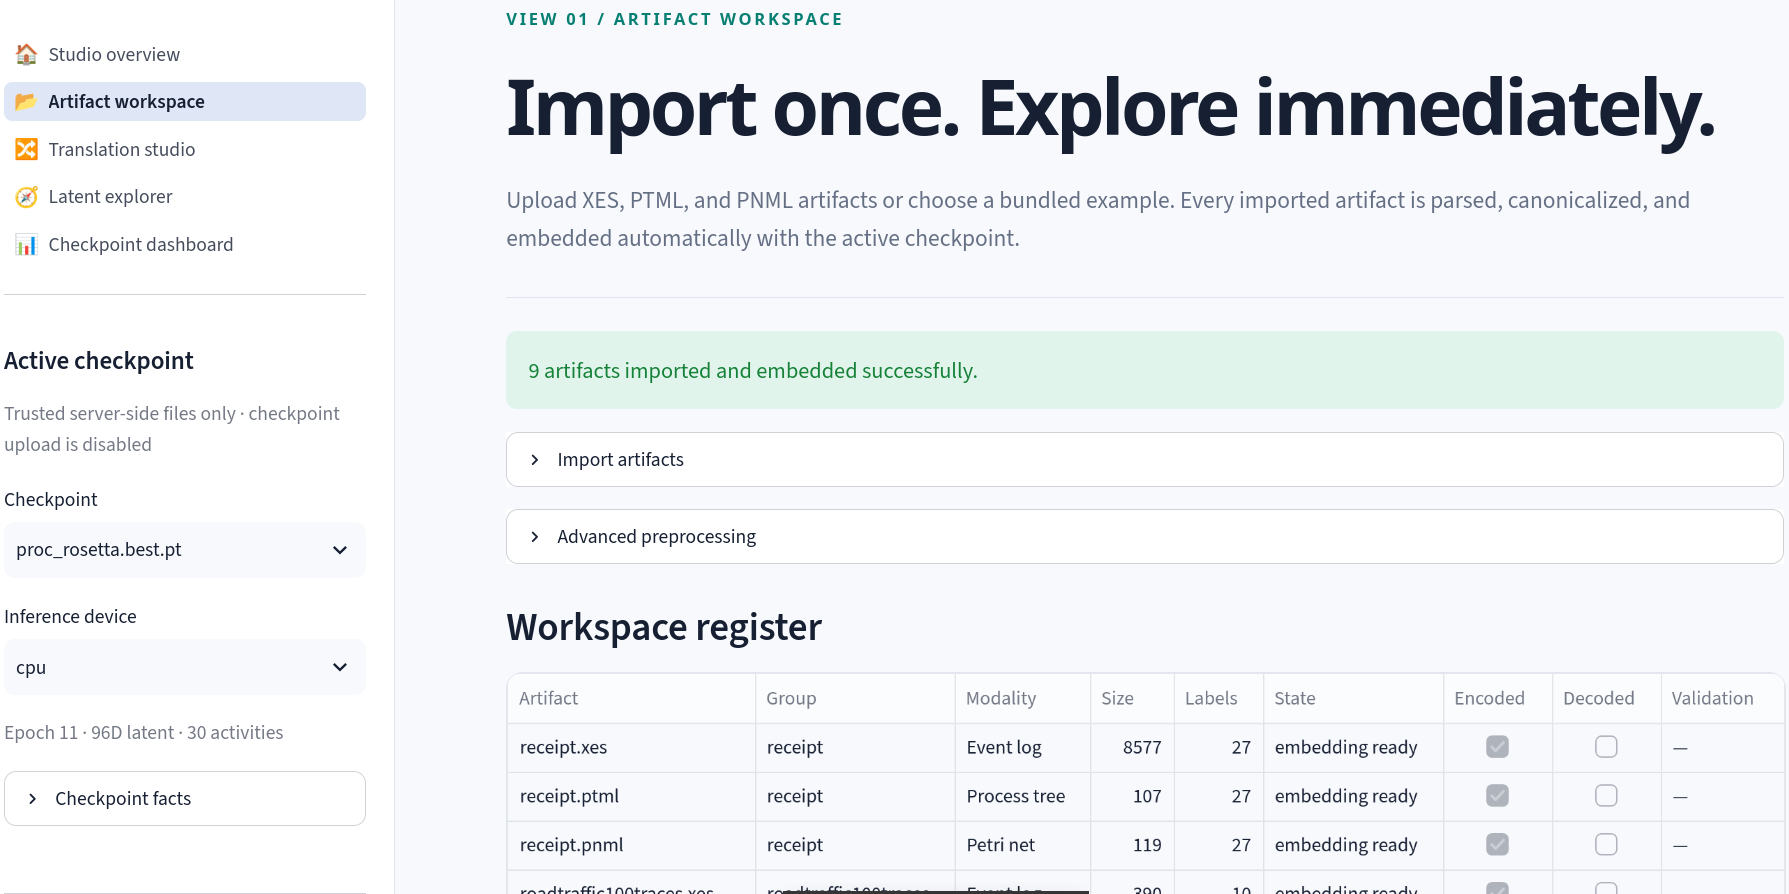
\includegraphics[width=\textwidth]{screenshots/rosetta-pm-artifact-workspace.png}
\caption{Artifact workspace of the public \model interface. XES, PTML, and PNML files are parsed, canonicalized, and embedded with the active checkpoint, while a shared register exposes the state and provenance of every imported artifact.}
\label{fig:tool-workspace}
\end{figure}

Second, the translation studio decodes either one artifact embedding or an equal-weight fusion of several selected embeddings. It exposes the token budget, source-activity constraint, and repeated-label policy, and it displays the grammar mask as the prefix is generated. Crucially, the result view in Fig.~\ref{fig:tool-translation} reports separate gates for end-of-sequence emission, grammar closure, operator arity, vocabulary, Petri-net convertibility, source-alphabet compliance, repeated labels, and length. This makes the distinction between syntactic validity and behavioral fidelity operational: users can inspect the restored-label tree, the deterministically derived Petri net, and source-versus-output comparisons instead of interpreting a successful parse as evidence of behavioral agreement. Outputs can be exported as PTML, a JSON validation report, derived PNML, or a simulated XES log.

\begin{figure}[H]
\centering
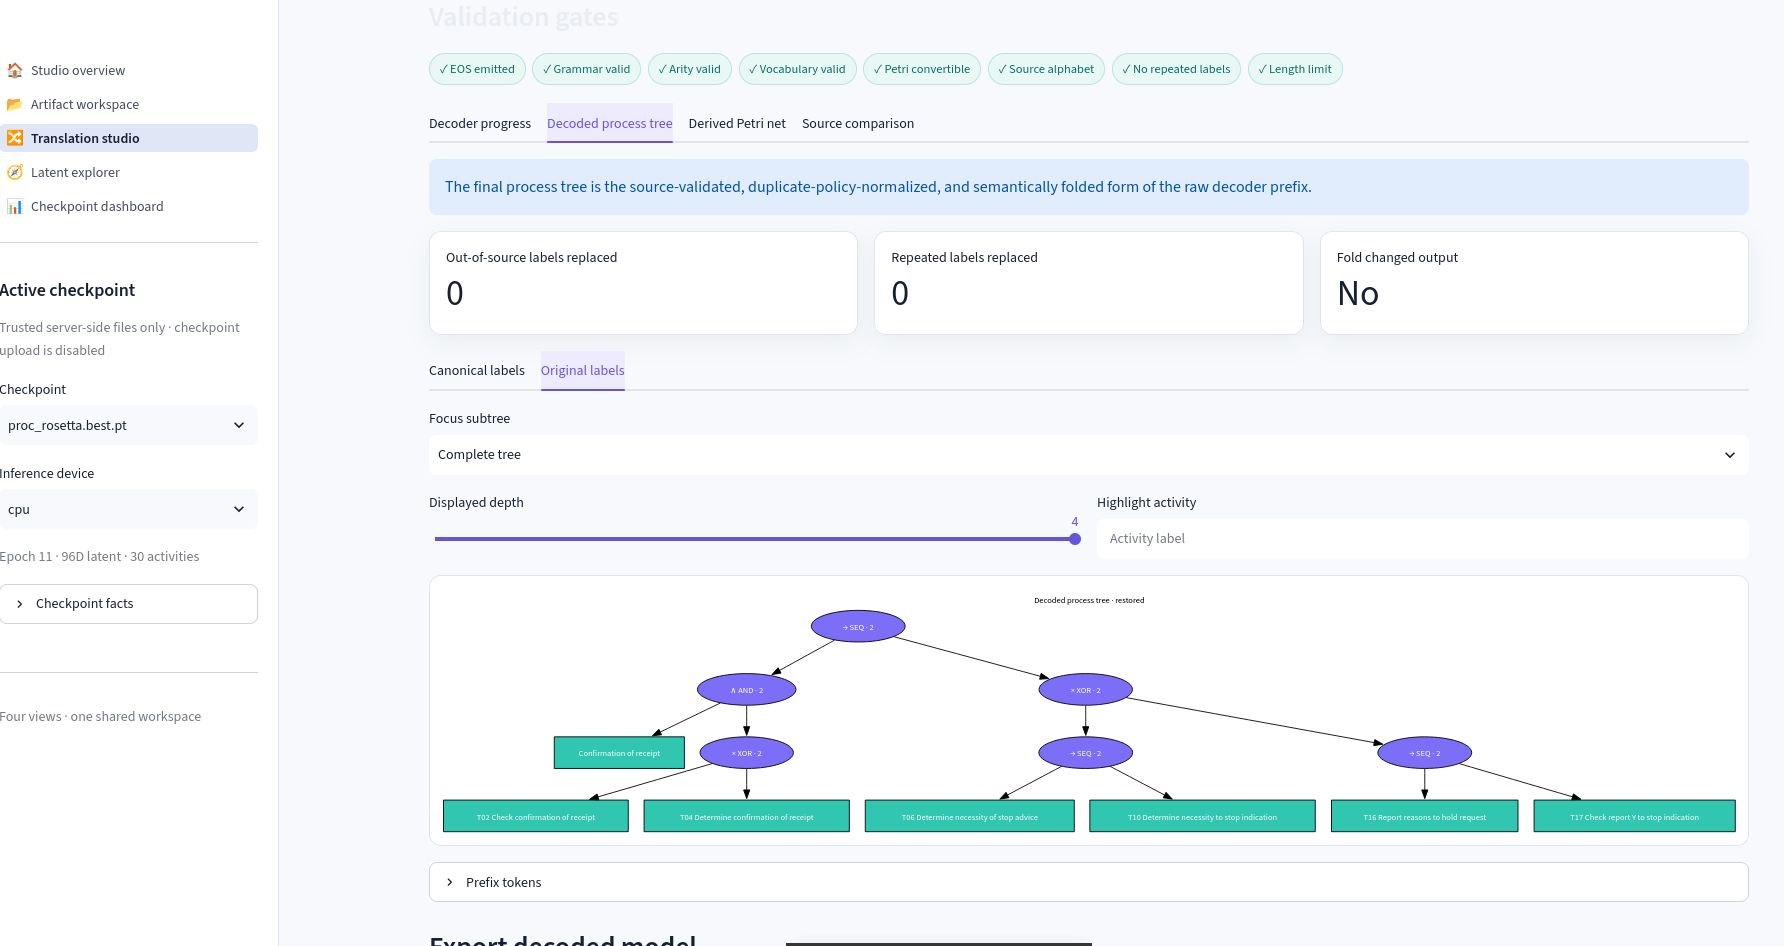
\includegraphics[width=\textwidth]{screenshots/rosetta-pm-translation-studio.png}
\caption{Translation studio after a constrained decode. Independent validation badges state exactly which guarantees passed; the selected tab visualizes the restored-label process tree, while adjacent views retain the decoder trace, derived Petri net, and source comparison.}
\label{fig:tool-translation}
\end{figure}

Third, the latent explorer in Fig.~\ref{fig:tool-latent} supports the representation-level use case that performs most strongly in the evaluation. It provides pairwise cosine similarity, PCA projection, process-group agreement, nearest-neighbor inspection, per-dimension views, latent interpolation, and a checkpoint-specific reference gallery. Equal-weight group means can be shown alongside the individual modalities, and vectors can be exported as JSON, CSV, or NumPy arrays. These views are diagnostic aids for investigating neighborhoods and failure cases; in particular, the two-dimensional PCA display is not used as a substitute for the quantitative retrieval and geometry protocols in Section~\ref{M-sec:results}.

\begin{figure}[H]
\centering
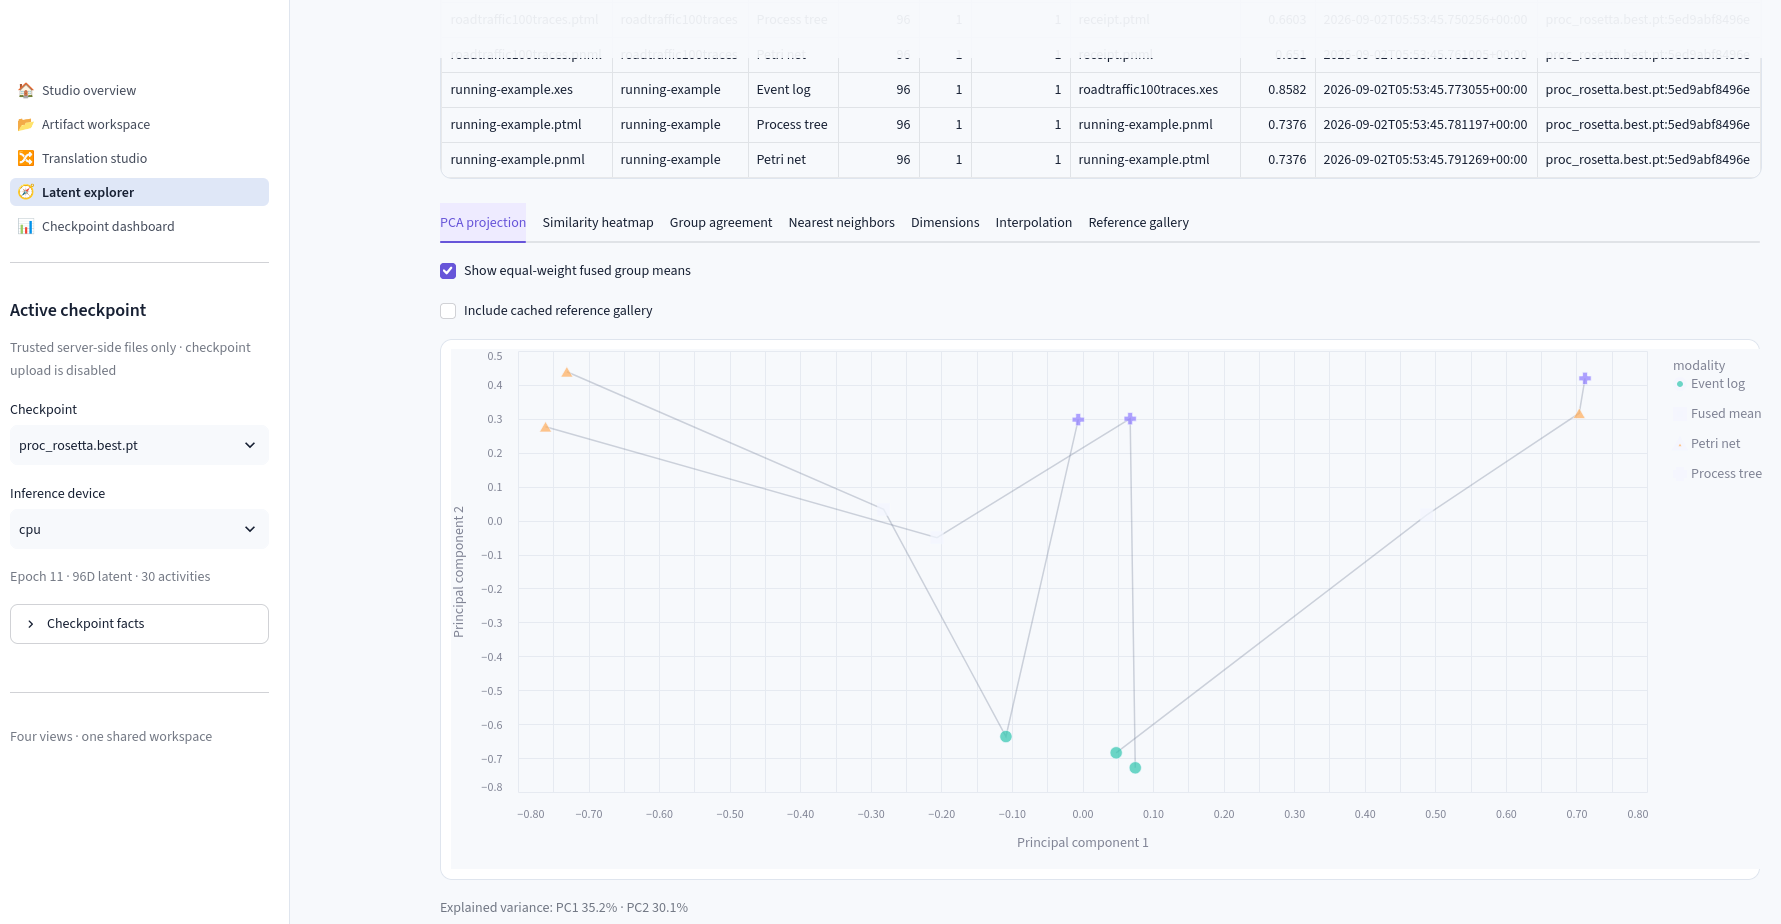
\includegraphics[width=\textwidth]{screenshots/rosetta-pm-latent-explorer.png}
\caption{Latent-space explorer with a PCA projection of event logs, process trees, Petri nets, and equal-weight fused group means. Connecting artifacts assigned to the same process group makes cross-artifact agreement and disagreement directly inspectable.}
\label{fig:tool-latent}
\end{figure}

\FloatBarrier
\subsection{Programmatic reproduction}

The command-line layer supports corpus generation, checkpoint training and evaluation, embedding export, and direct translation to PTML. External labels are canonicalized internally and restored after decoding whenever the source mapping is unambiguous. The corpus manifest, checkpoint provenance, machine-readable synthetic results, and real-log result record accompany the manuscript source. The principal reproduction commands are:

\begin{lstlisting}[basicstyle=\ttfamily\footnotesize,frame=single,breaklines=true]
./sample.py --data-dir data --train-families 4096 \
  --validation-families 512 --test-families 512 --seed 13 \
  --generator behavior_families --activity-vocab-size 30 \
  --traces-per-sample 128 --max-trace-length 128 \
  --variants-per-behavior 2 --log-views-per-behavior 2 \
  --log-view-modes uniform_variants,resampled
./train.py --data-dir data \
  --checkpoint checkpoints/proc_rosetta.pt \
  --epochs 100 --batch-size 128
./test.py --data-dir data --curriculum complex \
  --checkpoint checkpoints/proc_rosetta.best.pt --json
scripts/xes_to_ptml.py input.xes decoded.ptml \
  --checkpoint checkpoints/proc_rosetta.best.pt
python paper/generate_real_log_evaluation.py \
  --checkpoint checkpoints/proc_rosetta.best.pt
\end{lstlisting}

The training command sets a maximum horizon of 100 epochs. The reported run stopped after 17 completed epochs under the configured stopping policy, and epoch~11 was retained as the selected eligible checkpoint. In the test command, \texttt{--curriculum complex} selects only the complex test corpus; the simple and medium commands are run separately to produce the other result columns.

The last command repeats both duplicate-label policies on the fixed real-log samples, fits the Inductive Miner baselines, writes \texttt{real\_log\_evaluation.json}, and regenerates Fig.~\ref{M-fig:real-log-tree} as TikZ from PM4Py and Graphviz layout data. It does not create a PDF or raster asset. The repository README documents environment setup, the hosted and local browser interfaces, the trust boundary for checkpoints, and further import and export commands.

\FloatBarrier

\FloatBarrier

\section{Training details}\label{app:training-details}

Table~\ref{tab:loss-weights} resolves the conceptual objective groups in Section~\ref{M-sec:training} into the coefficients used by the selected checkpoint. The weights shown are the configured full-strength values; scheduled ramps and the source-specific adaptive reconstruction multipliers described in Section~\ref{M-sec:curriculum} are applied during training.

\begin{table}[H]
\centering
\caption{Complete objective coefficients for the selected checkpoint.}
\label{tab:loss-weights}
\begin{tabularx}{\textwidth}{@{}Yr@{\qquad}Yr@{}}
\toprule
Term & Weight & Term & Weight \\
\midrule
Tree reconstruction & 1.00 & Event-log reconstruction & 1.00 \\
Petri-net reconstruction & 1.00 & Fused reconstruction & 1.00 \\
Fused subset reconstruction & 0.25 & Constrained reconstruction & 0.25 \\
Exact cross-artifact contrast & 0.30 & Within-type contrast & 0.25 \\
Semantic exact contrast & 0.15 & Cross-batch memory contrast & 0.10 \\
Hierarchical metric ordering & 0.15 & Observation consistency & 0.15 \\
Soft behavioral geometry & 0.25 & Observed-distance regression & 0.20 \\
Observed-distance ranking & 0.20 & Latent alignment & 0.075 \\
Beam minimum-risk & 0.05 & Variance regularization & 0.10 \\
Covariance regularization & 0.01 & EOS / length / slots / completion & 0.05 each \\
Tree-complexity penalty & 0 & Duplicate-activity penalty & 0 \\
Kullback--Leibler & 0 & -- & -- \\
\bottomrule
\end{tabularx}
\end{table}

Table~\ref{tab:history} reports every completed epoch. The loss discontinuities at epochs 6 and 11 coincide with curriculum transitions and therefore do not compare the same training mixture.

\begin{table}[H]
\centering
\caption{Complete training history. Final-selection eligibility begins with the complex stage.}
\label{tab:history}
\begin{tabular}{@{}rrrrcr@{}}
\toprule
Epoch & Training loss & Validation loss & Selection score & Eligible & Learning rate \\
\midrule
1  & 5.179 & 10.018 & 0.595 & No  & $3.00\times10^{-4}$ \\
2  & 4.596 & 9.111  & 0.610 & No  & $3.00\times10^{-4}$ \\
3  & 5.028 & 6.693  & 0.643 & No  & $3.00\times10^{-4}$ \\
4  & 5.484 & 5.863  & 0.644 & No  & $3.00\times10^{-4}$ \\
5  & 6.109 & 5.472  & 0.679 & No  & $3.00\times10^{-4}$ \\
6  & 8.231 & 6.661  & 0.763 & No  & $3.00\times10^{-4}$ \\
7  & 7.904 & 6.136  & 0.707 & No  & $3.00\times10^{-4}$ \\
8  & 7.855 & 5.878  & 0.705 & No  & $1.50\times10^{-4}$ \\
9  & 7.633 & 5.716  & 0.715 & No  & $1.50\times10^{-4}$ \\
10 & 7.588 & 5.605  & 0.796 & No  & $1.50\times10^{-4}$ \\
11 & 9.194 & 7.794  & 0.787 & Yes & $1.50\times10^{-4}$ \\
12 & 9.162 & 7.550  & 0.703 & Yes & $1.50\times10^{-4}$ \\
13 & 9.137 & 7.412  & 0.713 & Yes & $7.50\times10^{-5}$ \\
14 & 9.449 & 7.334  & 0.707 & Yes & $7.50\times10^{-5}$ \\
15 & 9.040 & 7.284  & 0.721 & Yes & $3.75\times10^{-5}$ \\
16 & 9.144 & 7.241  & 0.716 & Yes & $3.75\times10^{-5}$ \\
17 & 8.919 & 7.220  & 0.719 & Yes & $1.875\times10^{-5}$ \\
\bottomrule
\end{tabular}
\end{table}

\FloatBarrier

\section{Running Example and Complete Serializations}\label{sec:supp-running}

The external running example demonstrates that the released interface can ingest all three supported file types and return process-tree output. It is a software-level illustration rather than an additional quantitative evaluation. Table~\ref{tab:running} summarizes the translations. Petri-net input produces the closest tree, but even direct process-tree reconstruction changes routing.

\begin{table}[H]
\centering
\caption{Running-example translation. Conformance compares each decoded process model with the source event log; lower tree edit and higher conformance indicate better agreement.}
\label{tab:running}
\begin{tabular}{@{}lrrrrrr@{}}
\toprule
Input & Output size & Depth & Tree edit $\downarrow$ & Fitness & Precision & F1 \\
\midrule
Source reference & 14 & 6 & 0.000 & 1.000 & 1.000 & 1.000 \\
Process tree & 16 & 6 & 0.360 & 0.474 & 0.360 & 0.409 \\
Event log & 14 & 5 & 0.545 & 0.737 & 0.400 & 0.519 \\
Petri net & 14 & 5 & \best{0.182} & \best{0.860} & \best{0.700} & \best{0.772} \\
\bottomrule
\end{tabular}
\end{table}

Figure~\ref{fig:running-example} compares the loop fragments of the source tree and the best decoded tree. The decoded version moves the decision and reinitiation sequence from the loop body/redo boundary. Section~\ref{app:serialized-example} gives the complete folded prefix forms for auditability.

\begin{figure}[H]
\centering
\resizebox{0.94\textwidth}{!}{%
\begin{tikzpicture}[
 panel/.style={draw=prgray!55,rounded corners=3pt,inner sep=5mm},
 op/.style={circle,draw,fill=prlightgold,minimum size=7mm,font=\scriptsize,inner sep=0pt},
 leaf/.style={draw,rounded corners=2pt,fill=prlightblue,minimum width=17mm,minimum height=6mm,font=\scriptsize,align=center},
 moved/.style={draw,rounded corners=2pt,fill=prlightred,minimum width=17mm,minimum height=6mm,font=\scriptsize,align=center},
 arr/.style={-{Stealth[length=1.5mm]},thin}
]
\begin{scope}[local bounding box=source]
\node[font=\small\bfseries] at (0,3.25) {Source loop fragment};
\node[op] (sl) at (0,2.55) {LOOP};
\node[op] (ss) at (-1.55,1.55) {SEQ};
\node[moved] (sr) at (1.75,1.55) {reinitiate};
\node[op,fill=prlightteal] (sa) at (-2.5,0.55) {AND};
\node[moved] (sd) at (-0.55,0.55) {decide};
\node[leaf] (sc) at (-3.45,-0.45) {check ticket};
\node[op] (sx) at (-1.45,-0.45) {XOR};
\node[leaf] (st) at (-2.4,-1.45) {examine\\thoroughly};
\node[leaf] (su) at (-0.5,-1.45) {examine\\casually};
\draw[arr] (sl)--(ss); \draw[arr] (sl)--(sr);
\draw[arr] (ss)--(sa); \draw[arr] (ss)--(sd);
\draw[arr] (sa)--(sc); \draw[arr] (sa)--(sx);
\draw[arr] (sx)--(st); \draw[arr] (sx)--(su);
\end{scope}
\node[panel,fit=(source)] {};

\begin{scope}[xshift=8.6cm,local bounding box=decoded]
\node[font=\small\bfseries] at (0,3.25) {Petri net-derived loop fragment};
\node[op] (dl) at (0,2.55) {LOOP};
\node[op,fill=prlightteal] (da) at (-1.7,1.55) {AND};
\node[op,fill=prlightred] (ds) at (1.7,1.55) {SEQ};
\node[leaf] (dc) at (-2.75,0.55) {check ticket};
\node[op] (dx) at (-0.85,0.55) {XOR};
\node[moved] (dd) at (0.75,0.55) {decide};
\node[moved] (dr) at (2.7,0.55) {reinitiate};
\node[leaf] (dt) at (-1.8,-0.45) {examine\\thoroughly};
\node[leaf] (du) at (0.1,-0.45) {examine\\casually};
\draw[arr] (dl)--(da); \draw[arr] (dl)--(ds);
\draw[arr] (da)--(dc); \draw[arr] (da)--(dx);
\draw[arr] (dx)--(dt); \draw[arr] (dx)--(du);
\draw[arr] (ds)--(dd); \draw[arr] (ds)--(dr);
\end{scope}
\node[panel,fit=(decoded)] {};

\node[draw=prred,fill=prlightred,rounded corners=2pt,font=\scriptsize] at (3.6,-2.95)
  {highlighted nodes cross the loop body/redo boundary};
\end{tikzpicture}%
}
\caption{Source and best decoded loop fragments for the running example; the common registration prefix and final choice are omitted. The decoded process tree moves \emph{decide} and \emph{reinitiate} into the loop's redo sequence.}
\label{fig:running-example}
\end{figure}


\FloatBarrier

\subsection{Complete Folded Prefix Serializations}\label{app:serialized-example}

The complete folded prefix forms underlying Table~\ref{tab:running} and Fig.~\ref{fig:running-example} are listed below.

\paragraph{Source tree.}
\begin{quote}\ttfamily\small\raggedright
SEQ(register request, LOOP(SEQ(AND(check ticket,
XOR(examine thoroughly, examine casually)), decide),
reinitiate request), XOR(reject request, pay compensation)).
\end{quote}

\paragraph{Decoded from process-tree input.}
\begin{quote}\ttfamily\small\raggedright
SEQ(register request, LOOP(AND(examine casually,
XOR(decide, AND(examine thoroughly, reinitiate request))),
SEQ(pay compensation, reject request)), XOR(tau, check ticket)).
\end{quote}

\paragraph{Decoded from event-log input.}
\begin{quote}\ttfamily\small\raggedright
SEQ(register request, XOR(examine casually,
AND(check ticket, decide, reinitiate request,
LOOP(examine thoroughly, pay compensation))),
XOR(tau, reject request)).
\end{quote}

\paragraph{Decoded from Petri-net input.}
\begin{quote}\ttfamily\small\raggedright
SEQ(register request, LOOP(AND(check ticket,
XOR(examine thoroughly, examine casually)),
SEQ(decide, reinitiate request)),
XOR(reject request, pay compensation)).
\end{quote}

\end{document}
